\chapter{OpenCvAda Benchmark}
\section{What we want to test:}
\subsection{Why test?}
Two of the major design goals in OpenCVAda are that the performance should be similar to OpenCV and operations on identical data should give the same result. To assert that these two goals are met several tests have been created to compare the execution time and output of different programs written identically in C, Python and Ada. 
\\
Running benchmarks and comparing the results of the samples provided with OpenCv compared to OpenCvAda versions of those samples, allows us to assume that the import to Ada does not change the performance or the results.
\subsection{Comparing OpenCvAda with OpenCv}
To make sure that OpenCvAda is comparable in speed and memory usage to OpenCv written with Python and C/C++, all the tests will have three versions one for each language.
\\
C/C++ is compiled as C++ using the compiler supplied with GNAT GPL 2010 (20100603).
Ada is compiled with the Ada compiler in GNAT GPL 2010 (20100603).
Python tests are executed using version 2.7.
\\
In Windows the OpenCv library is compiled with Visual Studio 2010 with Python and Qt\footnote{Qt\cite{qtweb} 4.7.1, LGPL version} support added, third party libraries are flagged to be rebuilt.
In Linux compilation is done with the standard compiler supplied with the distribution.
\subsection{Scaling of OpenCvAda}
OpenCvAda should be capable of handling applications with a larger scale then normal (example: large images) so three tests have been designed to measure performance on different cases where larger scales could be applied. This is to make sure that when importing OpenCv to Ada no issues arise on fringe cases due to memory leaks or related things. (example: OpenCvAda allocates data twice)
\subsection{Does the speed of OpenCvAda change in another OS}
This is to make sure that OpenCvAda is capable of running equal in both Windows and Unix-based systems in comparison with Python and C/C++. 
\subsection{Samples}
To make sure that OpenCvAda does not change the results of functions compared to OpenCv, a set of samples from OpenCv was implemented in Ada and the results are compared with the results of the OpenCv samples. This will catch any major problems with OpenCvAda compared to the OpenCv samples, or in a few cases find problems with the original samples.
\section{What we tested with:}
\subsection{The Benchmarker application}
The Benchmarker is an Ada application that uses Ada.Real_Time to time applications. To test any overhead with this application, we have the null tests that run empty applications in all three languages to measure the time needed to initialize.
\subsection{The Memory usage application}
The Memory usage application measures the memory allocated by different applications over time. The program was developed to compare the memory usage of applications written in different programming languages (C, Ada and Python) to assert that they behave in a similar way and also to detect potential memory leaks.
\\
Data is collected once per second and the lowest, highest and average memory usage is calculated and stored to later be saved together with each point of data gathered during execution.
\\
The data gathered is written to a comma-separated-value file to make it easier to import into a spreadsheet for a better overview and generate diagrams of the memory used over time.
\subsection{Platforms}
These operating systems will be tested:
\begin{itemize}
\item Windows 7\cite{win7}
\item Fedora Linux 14\cite{fedora}
\end{itemize}
The versions of OpenCv used is SVN revision 4784. The reason for using the SVN version is that certain elements (such as the use of web-cameras and videos) in OpenCV 2.2 (the latest release version) does not work in Windows 7. Using our own compiled version also allows the use of the improved QT version of Highgui in addition to fixing the broken things in version 2.2.
\subsection{Hardware}
The hardware used in the tests will be these computers:
\begin{itemize}
\item Lenovo X201 with built in camera.
\begin{itemize}
\item Windows 7 tests.
\item Fedora Linux 14 tests.
\end{itemize}
\item HP Pavilion dv3550eo with built in camera.
\begin{itemize}
\item Memory tests.
\end{itemize}
\end{itemize}
\subsection{Image and Video files used}
\begin{itemize}
\item heic0602a.jpg
\begin{itemize}
\item Dimensions: 15852x12392
\item Size: 62.1 mb
\item From NASA image gallery \cite{nasa}.
\end{itemize}
\item FlickAnmation.avi
\begin{itemize}
\item Dimensions: 300x250
\item Frames: 59
\item Size: 1,52 MB
\item Distributed with Windows 7.
\end{itemize}
\end{itemize}
\section{The actual tests:}
Several programs have been created to test the performance of OpenCVAda. This section describes each test and shows the results of the tests.
\subsection{Window creation}
This test was devised to check the overhead of the built-in window handler and general performance of loading and showing images in a window. The actual test consists of creating 100 windows through the Highgui package and showing an image in each window. After all the windows have been created they are all destroyed and the test finishes. The current implementation does not use the available function that destroys all created windows but instead iterates over each window and destroys them one by one. The reason for this is because at the time of implementation the Cv_Destroy_All_Windows function in OpenCV was not working as intended.
\begin{figure}
\centering
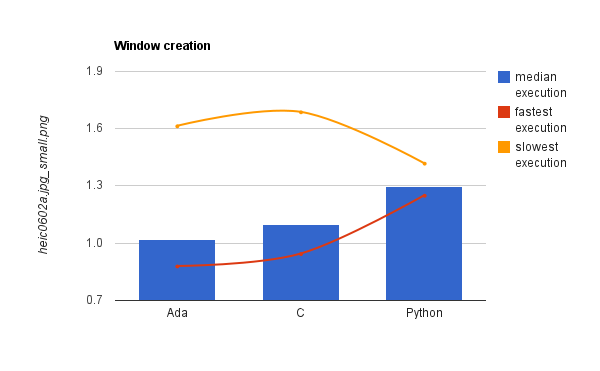
\includegraphics[width=1.0\textwidth]{GuiTestChart.png}
\caption{Benchmark of window creation and image loading.}
\label{fig:GuiTestChart}
\end{figure}
\\
Figure \ref{fig:GuiTestChart} shows the slowest, highest and average execution times for 100 executions of the program. As can be seen in the diagram, Ada performs slightly faster than C in all cases, whereas Python has the most stable albeit slowest execution times.
\subsection{Large image I/O}
This is a test of large file I/O and image operations, the program loads a large image file, re-sizes it and saves the re-sized image to the hard drive. The image used in this test has a resolution of 15852x12392 pixels and is re-sized to 640x480 pixels. 
\begin{figure}
\centering
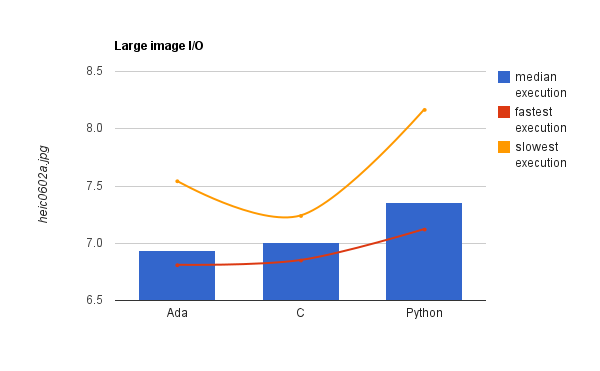
\includegraphics[width=1.0\textwidth]{bigTestChart.png}
\caption{Benchmark of operations on large images.}
\label{fig:bigTestChart}
\end{figure}
\\
The test application was run 100 times and the slowest, highest and average execution times are presented in Figure \ref{fig:bigTestChart}. As with the window creation test, Ada maintains the lowest average execution time compared to C and Python, although the difference in the average case between Ada and C is negligible.
\subsection{Algorithms}
This tests the performance of algorithms available in OpenCV on each frame in a video. The algorithms tested are a Canny edge detector and Hough transform to detect circles. This test can also be a good indicator of potential memory leaks due to the large number of images that are created and released. 
\\
The test was performed on a short video clip consisting of 59 frames at a 300x250 pixel resolution.
\begin{figure}
\centering
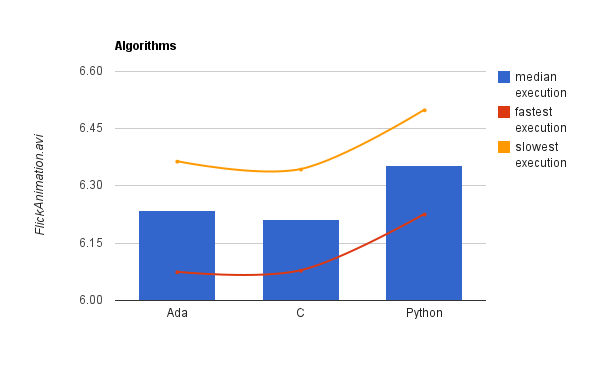
\includegraphics[width=1.0\textwidth]{LongTestChart.png}
\caption{Benchmark of image processing algorithms.}
\label{fig:LongTestChart}
\end{figure}
\\
The result of the algorithm test can be seen in Figure \ref{fig:LongTestChart}. Like the previous tests, the application was run 100 times and the slowest, highest, and average execution times are presented in the diagram. In contrast with the previous tests, C performs faster than Ada, although the the difference between the languages remains marginal.
\subsection{Memory usage}
This test is designed to compare the memory usage of applications. The applications used in this test are a subset of the samples supplied with OpenCV in C. The memory test can also be used to see if there are any memory leaks, which can be seen by an increasing use of memory over time in an application.
\\
A simple application is used as a reference for the memory usage difference between Ada and C, more information about this can be found in Executable reference(section \ref{sec:execref}).
\\
A subset of 4 sample applications were used to test how much memory they utilize over a 3 minute period, the results for each application in presented in the diagrams below. Each application has two diagrams associated with it, one diagram shows the highest, lowest and average memory usage and the second diagram shows the memory usage for each second of the execution.
The subset of applications consist of the following:
\begin{itemize}
\item Delaunay triangulation - Generates random Delaunay triangulations.
\item Farneback optical flow - Displays the optical flow from a live camera feed.
\item Motion - Tracks objects motion from a live camera feed.
\item Polar transform - Does a polar transform on images from a live camera feed and then reconstructs the image.
\end{itemize}
\begin{figure}
\centering
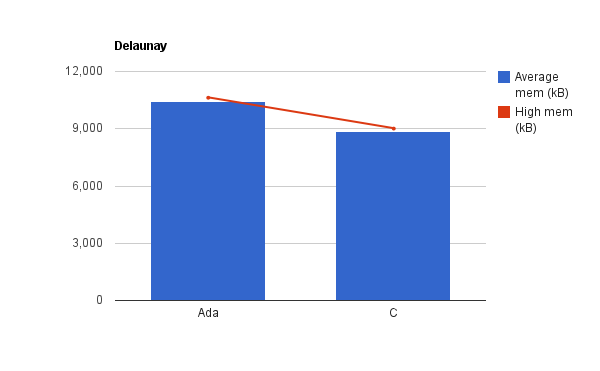
\includegraphics[width=1.0\textwidth]{memdelaunay.png}
\caption{Overall memory usage of Delaunay triangulation.}
\label{fig:memdelaunay}
\end{figure}
\begin{figure}
\centering
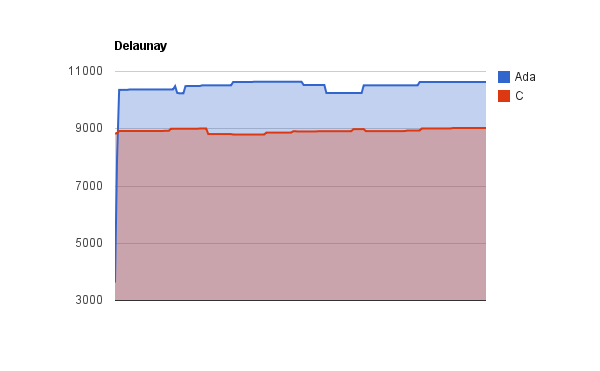
\includegraphics[width=1.0\textwidth]{MemUseDelaunay.png}
\caption{Memory usage per second of Delaunay triangulation.}
\label{fig:MemUseDelaunay}
\end{figure}
The memory usage of the Delaunay triangulation in OpenCVAda is on average 17 percent higher than its OpenCV counterpart as can be seen in Figure \ref{fig:memdelaunay}. Figure \ref{fig:MemUseDelaunay} shows that the behaviour of memory allocation is similar in both OpenCV and OpenCVAda.
\begin{figure}
\centering
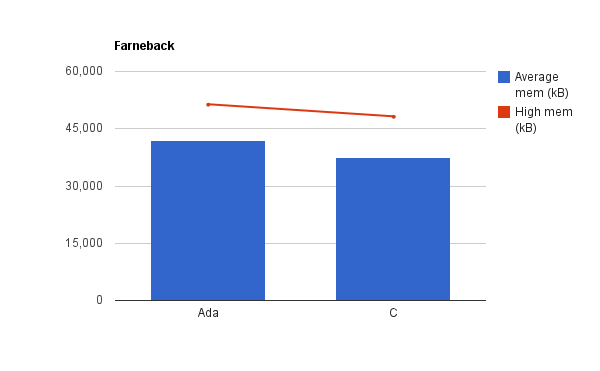
\includegraphics[width=1.0\textwidth]{memfarneback.png}
\caption{Overall memory usage of Farneback optical flow.}
\label{fig:memfarneback}
\end{figure}
\begin{figure}
\centering
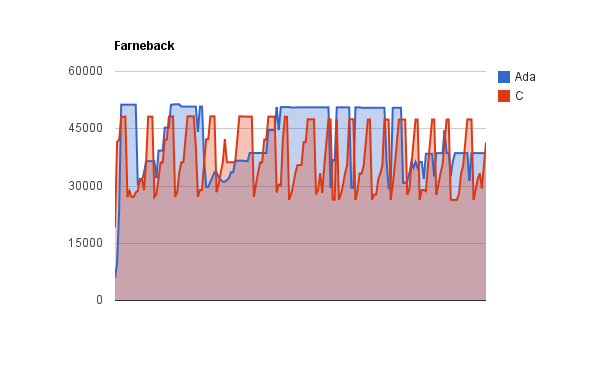
\includegraphics[width=1.0\textwidth]{MemUseFarneback.png}
\caption{Memory usage per second of Farneback optical flow.}
\label{fig:MemUseFarneback}
\end{figure}
\\Figure \ref{fig:memfarneback} shows again that the memory usage in OpenCVAda is higher than OpenCV, 11 percent more memory is used on average. Figure \ref{fig:MemUseFarneback} shows the similarity of the memory allocation behaviour throughout the execution. The reason why the curves look different is because the application constantly allocate and release images and as a result the memory information from OpenCVAda was polled at peaks more often than OpenCV.
\begin{figure}
\centering
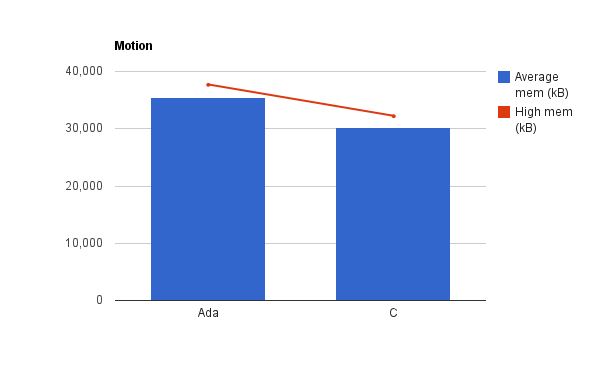
\includegraphics[width=1.0\textwidth]{memmotion.png}
\caption{Overall memory usage of motion tracker.}
\label{fig:memmotion}
\end{figure}
\begin{figure}
\centering
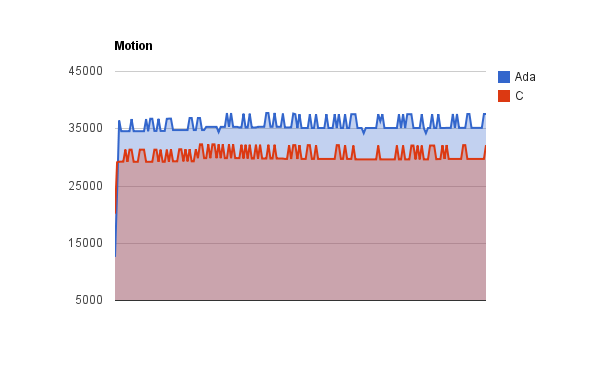
\includegraphics[width=1.0\textwidth]{MemUseMotion.png}
\caption{Memory usage per second of motion tracker.}
\label{fig:MemUseMotion}
\end{figure}
\\As with the previous applications, Figure \ref{fig:memmotion} show that OpenCVAda use more memory than OpenCV. Approximately 10 percent more memory is used when the application is execute through OpenCVAda. Figure \ref{fig:MemUseMotion} shows that the behaviour of the applications memory is very similar.
\begin{figure}
\centering
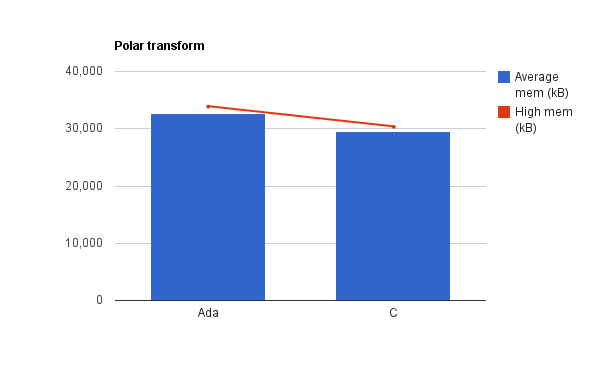
\includegraphics[width=1.0\textwidth]{mempolar}
\caption{Overall memory usage of polar transformation.}
\label{fig:mempolar}
\end{figure}
\begin{figure}
\centering
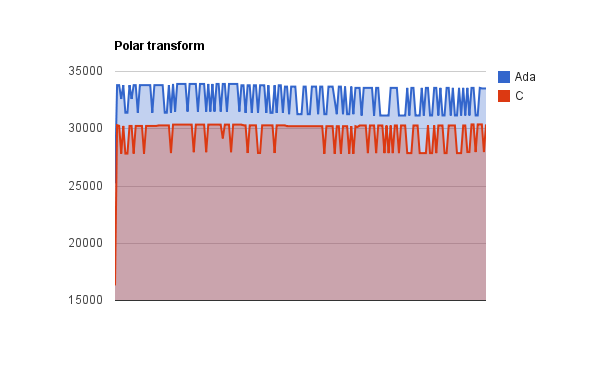
\includegraphics[width=1.0\textwidth]{MemUsePolar.png}
\caption{Memory usage per second of polar transformation.}
\label{fig:MemUsePolar}
\end{figure}
\\In the final test OpenCVAda utilize more memory yet again, as can be seen in Figure \ref{fig:mempolar} approximately 17 percent more memory is used in OpenCVAda compared to OpenCV. The memory allocation is behaving in a similar manner in both OpenCVAda and OpenCV which is shown in Figure \ref{fig:MemUsePolar}.
\subsection{Linux}
Comparing the execution time of the Window creation and Large image I/O between Linux and Windows, this allows for a base comparison between the operating systems. The results can be seen in Figure \ref{fig:linuxguichart} and \ref{fig:linuxbigchart}.
\begin{figure}
\centering
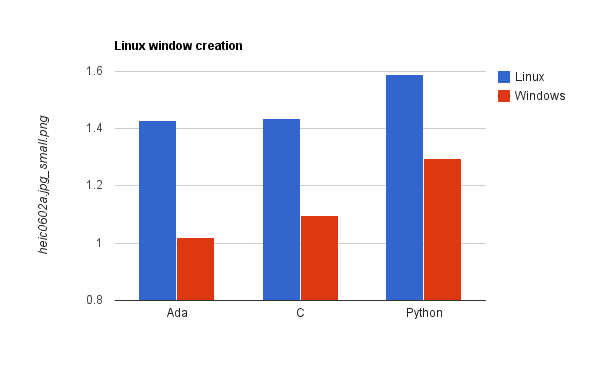
\includegraphics[width=1.0\textwidth]{linuxguichart.png}
\caption{Comparison of Linux and Windows window creation}
\label{fig:linuxguichart}
\end{figure}
\begin{figure}
\centering
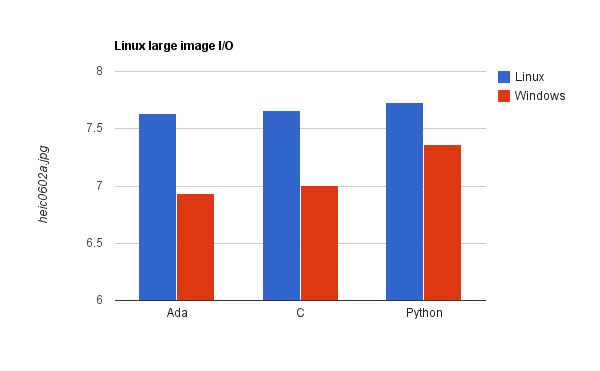
\includegraphics[width=1.0\textwidth]{linuxbigchart}
\caption{Comparison of Linux and Windows large image I/O}
\label{fig:linuxbigchart}
\end{figure}
\\Without a deeper analysis of Fedora Linux execution times it is hard to take anything away fro these diagrams except that compared to Windows the executions in Linux are much closer between languages then in Windows, however the same trends can be seen with Ada being the fastest close to C and Python coming in last with a margin. If we look at Executable reference (section \ref{sec:execref})  we will see that the execution time is not related to Linux applications being slower and it is more likely that the culprit lies in the compiler and or settings used to compile the OpenCv libraries. Other variables could range from GTK/QT differences to file systems and without more data it is impossible to give a more exact picture. The important part of the data in the scoop of this report is that in both Linux and Windows have OpenCvAda execution times very close to OpenCv C.
\subsection{Executable reference}\label{sec:execref}
To get reference data this test was designed to execute an empty application from Ada, C and Python in both Windows and Linux. This test is used as a baseline and also to make sure that the other tests are not influenced by the language or platform to a large degree. As we can see in the diagrams the overhead caused in choice of language and platform is negligible, this means that the platform and language can be chosen on other merits then performance unrelated to OpenCv. The tests results can be seen for Windows in Figure \ref{fig:NullTestChart} and Linux in Figure \ref{fig:linuxnullchart}.
\begin{figure}
\centering
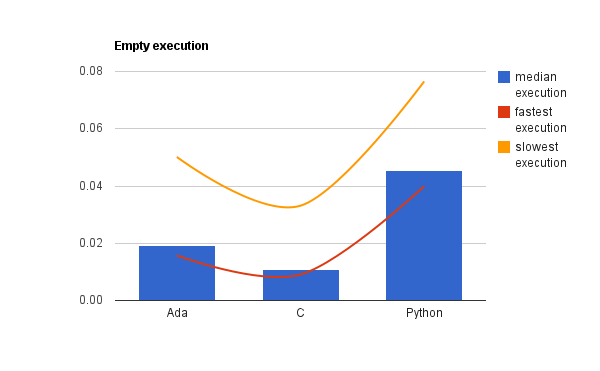
\includegraphics[width=1.0\textwidth]{NullTestChart}
\caption{Benchmark of Windows reference.}
\label{fig:NullTestChart}
\end{figure}
\begin{figure}
\centering
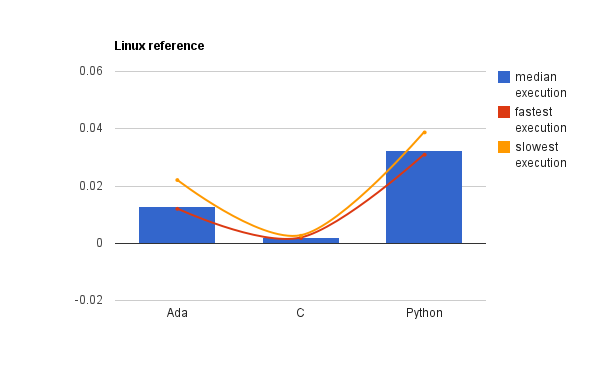
\includegraphics[width=1.0\textwidth]{linuxnullchart}
\caption{Benchmark of Linux reference.}
\label{fig:linuxnullchart}
\end{figure}
\\
Memory usage varies between programming languages and compilers, different languages allocate different resources to optimize execution times and other functionality. The representation of data is also different between languages which influences the memory usage.
\\
A simple application (an infinite loop that prints the numbers 0-100) was implemented in Ada and C and the memory usage of both applications was measured to get a baseline for difference in memory usage between the languages.
\\
\begin{figure}
\centering
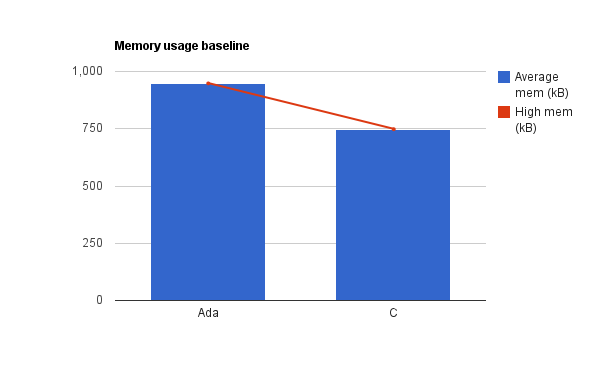
\includegraphics[width=1.0\textwidth]{membaseline.png}
\caption{Memory usage baseline reference.}
\label{fig:membaseline}
\end{figure}
The test in Figure \ref{fig:membaseline} shows that Ada in this case utilize approximately 25 percent more memory than C. Although the test is very simplistic, the memory difference percentage will be used as a criteria for assessing the memory usage of the OpenCVAda samples compared to their OpenCV equivalent.
\subsection{Correctness}
By taking the samples supplied with OpenCV and re-implementing them in OpenCVAda it is possible to compare the results from both libraries. If the results are not identical there is some problem that needs to be isolated and repair. In order to get identical results it is not possible to use a live camera to capture frames to process, a video clip will be used instead. Some of the OpenCV samples have a problem with video playback, in these cases a live camera capture was used instead and as a result it is not possible to simply compare the output. In these cases the assessment will be based on the general functionality and similarity of the output.
\\
This test involves the samples supplied with OpenCv and the ported versions in OpenCvAda and comparing the results of the executions of the samples. This should show any major errors with the imported functions from C.
\\
Due to issues with the video play back in OpenCv (C/C++, Python) samples, in some cases (figure Alpha and figure Delta) where a video file could be used a camera is used instead. So those samples needs to be compared for the actual functionality and not only the results.
\\
We decided on presenting a subset of the samples and the results here for comparing the OpenCvAda samples with OpenCv. The Figures are \ref{fig:bgfg}, \ref{fig:findobj}, \ref{fig:latentsvm},\ref{fig:motempl} and \ref{fig:mser}.
\begin{figure}
\centering
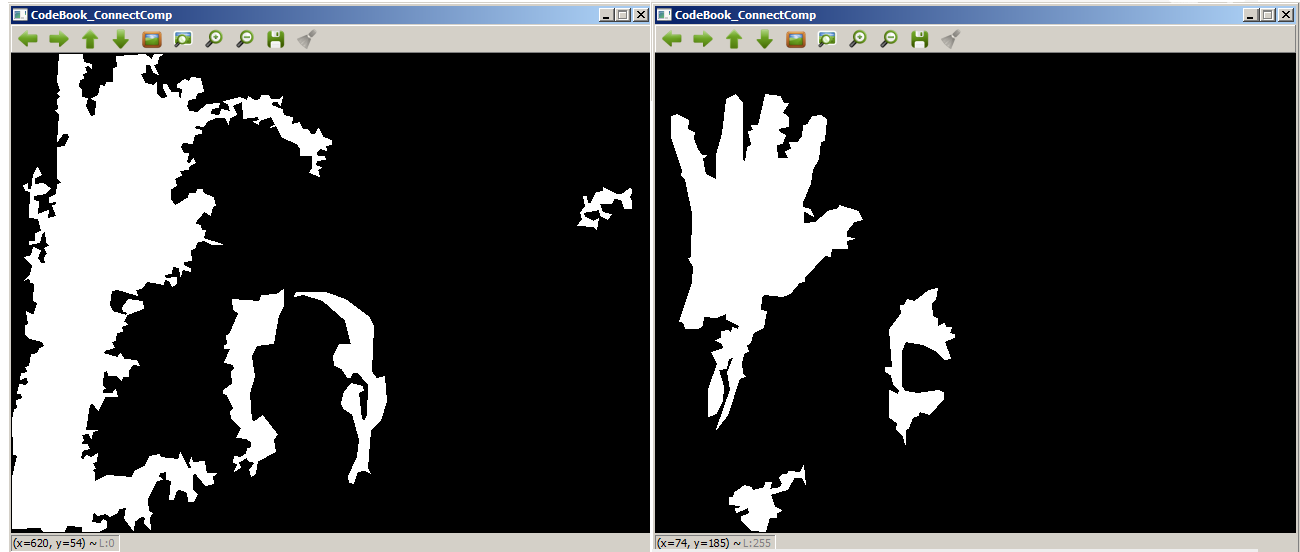
\includegraphics[width=1.0\textwidth]{bgfg}
\caption{Comparison of bgfg_codebook sample.}
\label{fig:bgfg}
\end{figure}
\begin{figure}
\centering
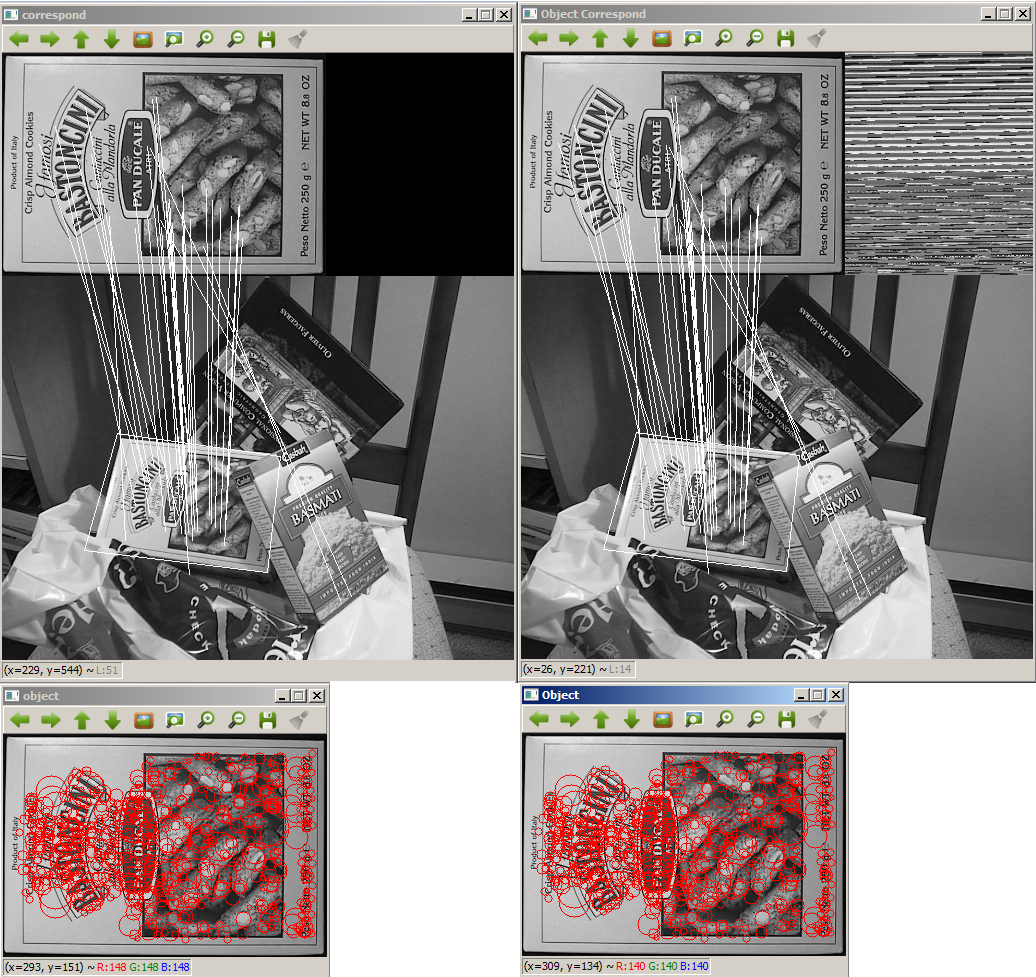
\includegraphics[width=1.0\textwidth]{findobj}
\caption{Comparison of find_object sample.}
\label{fig:findobj}
\end{figure}
\begin{figure}
\centering
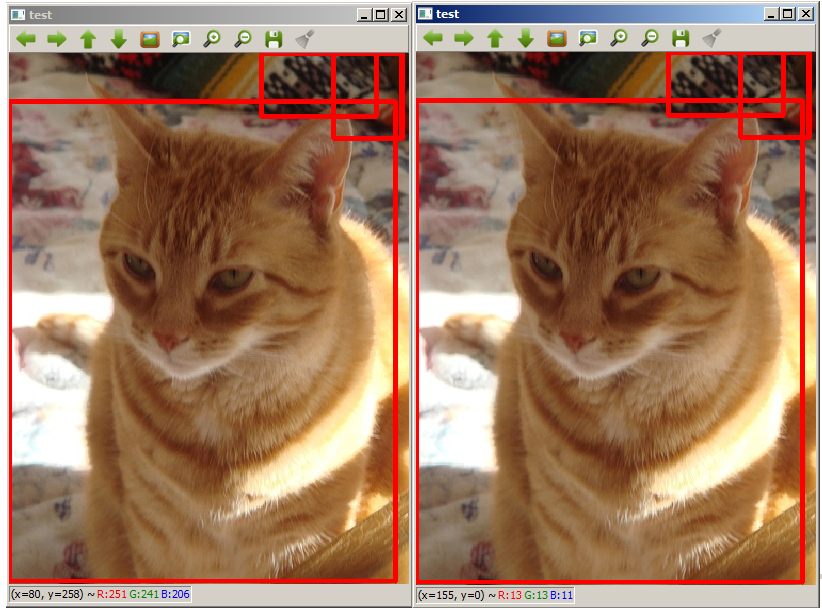
\includegraphics[width=1.0\textwidth]{latentsvm}
\caption{Comparison of latentsvm sample.}
\label{fig:latentsvm}
\end{figure}
\begin{figure}
\centering
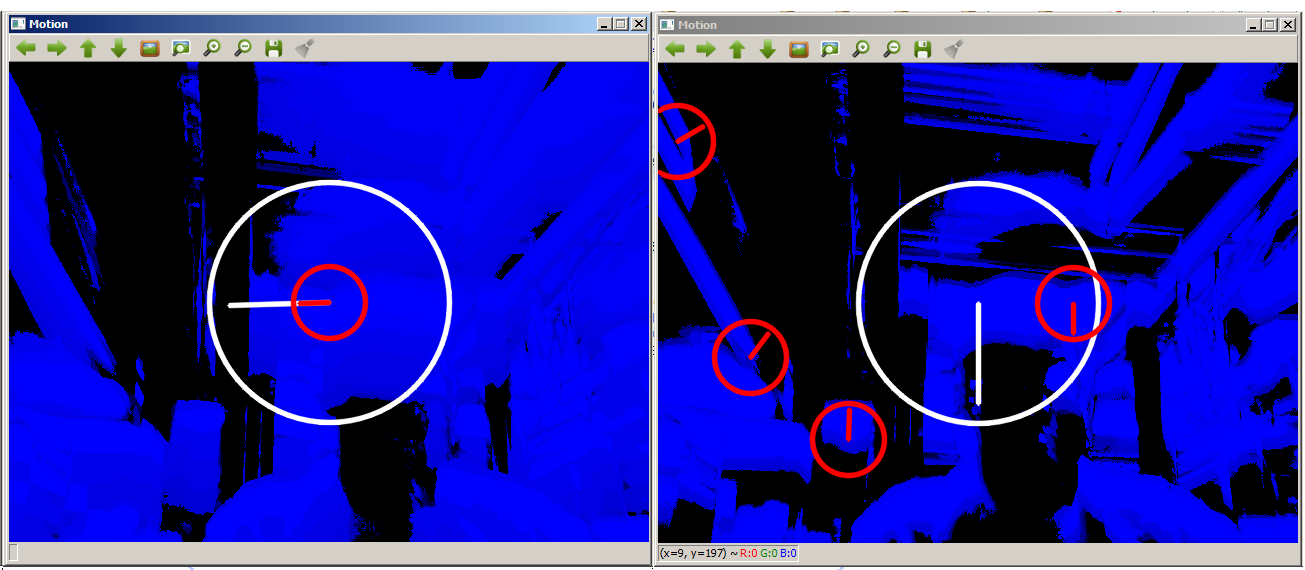
\includegraphics[width=1.0\textwidth]{motempl}
\caption{Comparison of motempl sample.}
\label{fig:motempl}
\end{figure}
\begin{figure}
\centering
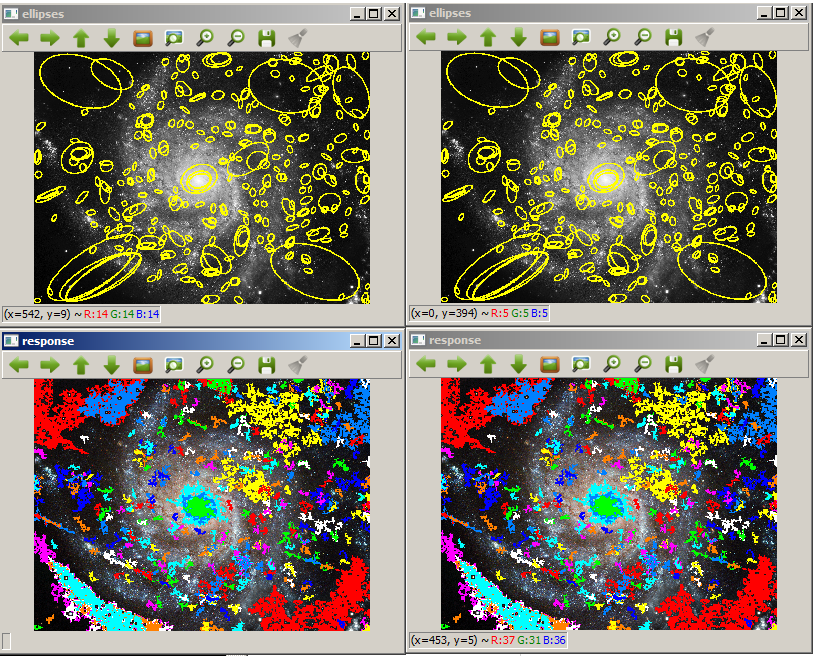
\includegraphics[width=1.0\textwidth]{mser}
\caption{Comparison of mser sample.}
\label{fig:mser}
\end{figure}
\section{Benchmark Results}
Performance of OpenCvAda in Windows 7 is better then expected with OpenCvAda having slightly lower average execution time then the C code in two out of three test cases. As a reference we can look at the execution of an empty application in each language to see that Ada is not always faster then C. Even though OpenCvAda can not be considered a huge performance boost it can not be consider a performance liability either, this allows for the language with the best features for the application to be chosen instead of performance dictating which language should be used. So regarding performance we can summarise it as avoid Python if performance is a key factor but the choice of Ada or C will not hugely impact performance. Similar results can be seen in Linux but with the reservation that OpenCvAda in Windows 7 is showing better performance in the benchmarks.
\\
The correctness test is used as more of a internal test that was used during implementation of OpenCvAda to make sure that OpenCvAda does not break any functionality from OpenCv and that a port between the two is not too complicated. If we look at both the complexity of the samples compared to the OpenCv version and the functionality, OpenCvAda can be considered according to the results found an equal version compared to the C version.
\\
The memory management in OpenCVAda is less efficient than OpenCV, in the best case approximately 10 percent and in the worst case 17 percent more memory was used. The average memory use over all four applications were 14.24 percent higher than OpenCV. All of the results are within the criteria specified in Executable reference (section \ref{sec:execref}).
